\documentclass[
fontsize=12pt,
paper=a4,
parskip=false
]{article}
\usepackage[right=20mm]{geometry}
\usepackage{todonotes}
\usepackage[ngerman]{babel}
\usepackage{ucs}                                                                 
\usepackage[utf8x]{inputenc} 
\usepackage{multirow,tabularx}
\usepackage{hhline}
\usepackage{caption}
\captionsetup{labelformat=empty}
\usepackage{array}
\newcolumntype{C}[1]{>{\centering\let\newline\\\arraybackslash\hspace{0pt}}m{#1}}
\usepackage{csquotes}
\captionsetup[figure]{font=small,skip=0pt}


\begin{document}
	\noindent\makebox[\linewidth]{\rule{\textwidth}{0.4pt}}
	Rebekka Rupprecht, Informatik \textit{Master of Science} \hfill \today \newline
	Deep Learning Lab Course \newline
	Report Exercise 3 \newline
	\noindent\makebox[\linewidth]{\rule{\textwidth}{0.4pt}}
	\vspace{5pt}

\section*{Implementing a decoder module for Fully Convolutional Networks}
In the first four pictures we can see the Intersection over Union plot for the different configuration. The first configuration consists of a upsampling function which produces 120 output features, which are 16x bigger in resolution than input. 

In the second configuration there is a refinement block  implemented, which adds so called skip connections from the encoder part to the decoder part. These skip connections provide information for reconstructing accurate shapes for segmentation boundaries. 

Third configuration uses two skip connection processings and in the last configuration there are all skip connections processed. 

On x-axis in the plots we can see the epoch number and on the y-axis the Intersection over Unit. 
\begin{figure}[ht] 
	\label{fig7} 
	\begin{minipage}[b]{0.6\textwidth}
		\centering
		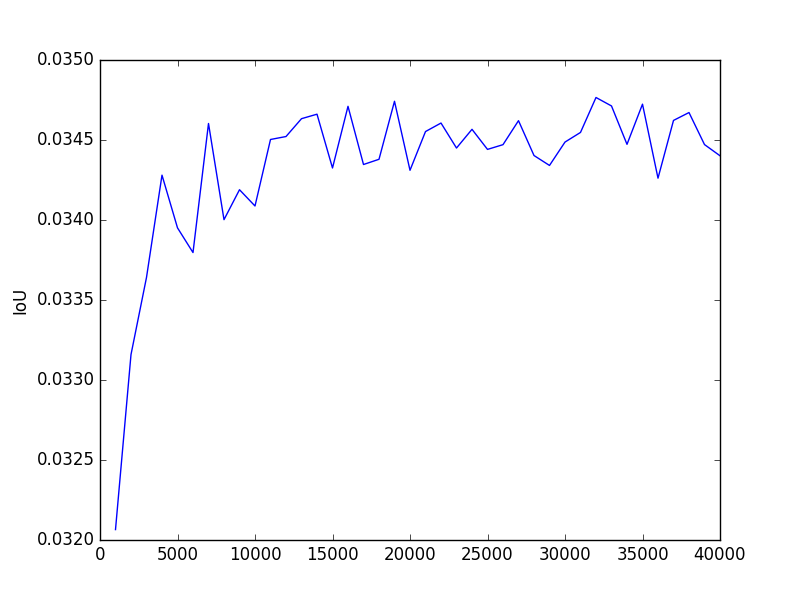
\includegraphics[width=.6\textwidth]{config_1} 
		\caption{Configuration 1} 
	\end{minipage}%%
	\begin{minipage}[b]{0.6\textwidth}
		\centering
		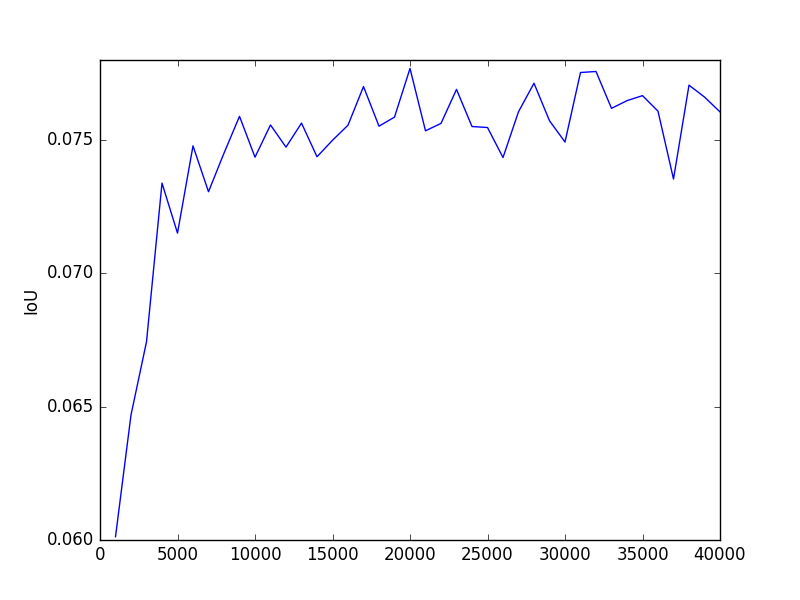
\includegraphics[width=.6\textwidth]{config_2} 
		\caption{Configuration 2} 
	\end{minipage} 
	\begin{minipage}[b]{0.6\linewidth}
		\centering
		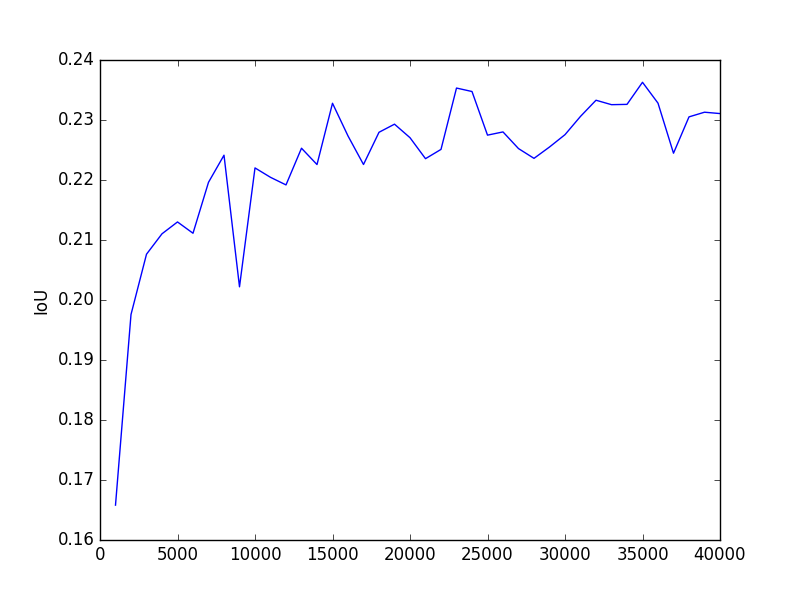
\includegraphics[width=.6\linewidth]{config_3} 
		\caption{Configuration 3} 
	\end{minipage}%% 
	\begin{minipage}[b]{0.6\linewidth}
		\centering
		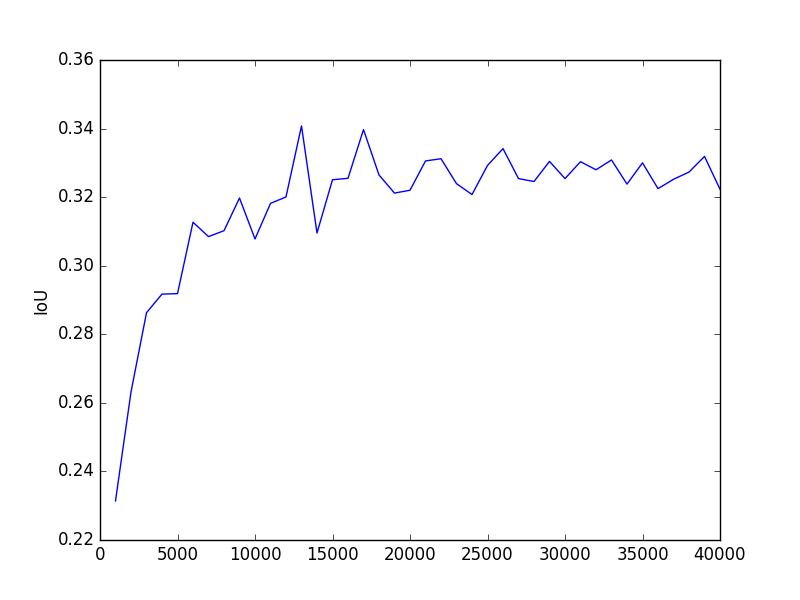
\includegraphics[width=.6\linewidth]{config_4} 
		\caption{Configuration 4} 
	\end{minipage} 
\end{figure}

In picture \ref{allConfigs} we can see all four configurations' IoUs in one plot. Here we can easily see that configuration 4, which is the only one processing skip connection 2,3 and 4, is the best one. 

\begin{figure}[ht]
\centering 
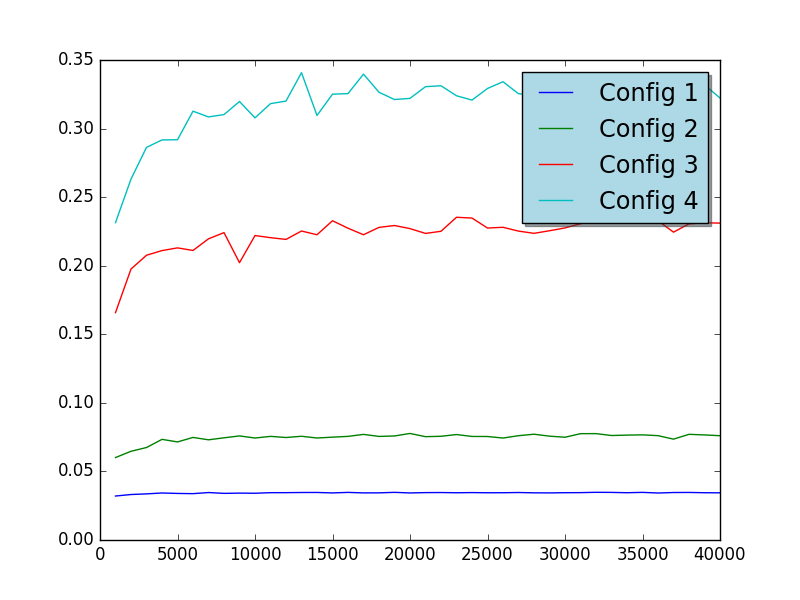
\includegraphics[width=0.8\textwidth]{allConfig}
\caption{All Configuration}
\label{allConfigs}
\end{figure}
\newpage
In table \ref{table} we can also see configuration 4 is the one with the highest Maximum IoU. 
\begin{table}[h!]
\centering
\begin{tabular}{|c|c|}
	\textbf{Configuration} & \textbf{Maximum IoU} \\
	\hline
	Configuration 1 & 3.48 \% \\
	Configuration 2 & 7.77 \% \\
	Configuration 3 & 23.63 \% \\
	Configuration 4 & 34.08 \% \\
\end{tabular}
\caption{Comparison Maximum IoU}
\label{table}
\end{table}
\end{document}